\chapter{THEORETICAL FRAMEWORK}

In this chapter, we present and discuss the tools and methodology utilized to build \emph{Scandal}. We start discussing how to produce sound in the Java Runtime Environment, and particularly how it deals with real-time audio. We next give a formal presentation on how the domain-specific language was designed, and attempt to classify it among other programming languages and music-DSL's. Finally, we address the methodology involved in building its compiler, appending to the latter a short discussion on how a general-user interface was designed to provide an integrated development environment experience for the end user, as well as alternative command-line methods for compiling and running \emph{Scandal} programs.

\section{How \emph{Scandal} Manages Sound}

The JRE System Library provides a very convenient package of classes that handle the recording and reproduction of real-time audio, namely the \il{javax.sound.sampled} package. In it, we find two classes, \il{TargetDataLine} and \il{SourceDataLine}, that deal respectively with capturing audio data from the system's resources, and playing back buffers of audio data owned by the application. An instance of \il{SourceDataLine} provides a \il{write} method that takes three arguments: an array of bytes to written to a \il{Mixer} object, an integer offset, and an integer length. In \emph{Scandal}, we do not specify a \il{Mixer} object, hence we make use of one provided by the \il{System}. There are two main aspects of the \il{write} method that need to be addressed. Firstly, it blocks the thread in which it lives until the given array of bytes has been written, from offset to length, to the \il{Mixer} its \il{SourceDataLine} contains; secondly, if nothing is done, it returns as it has no more data to write. In order to have real-time audio, one then needs to be constantly feeding this \il{write} method with audio samples, for as long as one wants continuous sound output, even if these buffers of audio samples contain only zeros, i.e., silence. It immediately follows that one must specify exactly how many samples are sent at a time, naturally with consequences to the system's performance. This parameter is commonly referred in the industry as the \emph{vector size}. The trade-off is measured in terms of latency: a large a vector size helps slower systems perform better, or can allow more complex processing, or even increase polyphony. Latency, however, is bad for any live application, including the generation of MIDI notes, and the recording of live sound from a microphone. A good, low-compromise vector size is usually set to 512 samples, and normally these sizes will be powers of two. In order to specify the preferred vector size, as well as many other environment settings, \emph{Scandal} refers to a static class named \il{Settings}, which contains a static property \il{Settings.vectorSize}.

The aforementioned two characteristics of the \il{write} method within a \il{SourceDataLine} are managed by \emph{Scandal} by the class \il{AudioFlow}. In order to prevent \il{write} from prematurely returning, an instance of \il{AudioFlow} contains a boolean property named \il{running}, which is set to \il{true} for as long as real-time audio is desired. The fact that \il{write} blocks its thread, however, is managed by any class that contains itself an instance of \il{AudioFlow} as a property. The latter are in \emph{Scandal} the implementors of the \il{RealTimePerformer} interface, which is a contract that contains four abstract methods: \il{startFlow}, \il{stopFlow}, \il{getVector}, and \il{processMasterEffects}. The role of the \il{startFlow} is to merely embed an \il{AudioFlow} within a new \il{Thread} object and start this new thread. This guarantees the thread that manages audio is different than the main \il{Application} thread, hence resolving the thread-blocking issue. Once a new \il{Thread} is started in \emph{Java}, however, one cannot in general interrupt it. In order to stop the audio thread, we set the property \il{running} inside an \il{AudioFlow} to false via the \il{stopFlow} method, which causes the \il{write} method inside the \il{AudioFlow} to return. Hence one cannot resume an audio process in \emph{Scandal} at this point, even though doing so is perfectly possible in \emph{Java}. The reason for that is not that of a design choice, but rather the fact that the domain-specific language is at its infancy, and many important features that go beyond a proof-of-concept are yet to be implemented. The \il{getBuffer} method is called by the \il{AudioFlow} every time it needs to write another vector of audio samples. It is the responsibility then of any \il{RealTimePerformer} to timely compute the next \il{Settings.vectorSize} samples of audio data. Finally, the \il{processMasterEffects} routine is called from within \il{getVector} to further process the buffer of audio samples. This is usually done while the samples are still represented as floats, hence before converting them to raw bytes.

The constructor of an \il{AudioFlow} takes, in addition to a reference to a \il{RealTimePerformer}, a reference to an \il{AudioFormat} object. The latter is part of the \il{javax.sound.sampled} package and is how we ask the \il{AudioSystem} for a \il{SourceDataLine}. Instead of constructing \il{AudioFormat} objects, however, the \il{Settings} class contains static members \il{Settings.mono} and \il{Settings.stereo} that are instances of \il{AudioFormat} defining a mono and stereo format, respectively. In addition to a channel count argument, \il{AudioFormat} instances are constructed by specifying a sampling rate, and a bit depth (word length) for audio samples. Those are, too, static properties in the \il{Settings} class, namely \il{Settings.samplingRate} and \il{Settings.bitDepth}. Listing \ref{alg:play} gives the specifics of maintaining a \il{SourceDataLine} open inside an instance of \il{AudioFlow}. The latter implements, in turn, the \il{Runnable} interface, hence needs to override a \il{run} method. Inside this \il{run} method, we call the private \il{play} subroutine that is given below:

\begin{lstlisting}[language=Java,caption={Writing buffers of audio data inside the \il{play} subroutine.},label={alg:play}]
private void play() throws Exception {
	SourceDataLine sourceDataLine = AudioSystem.getSourceDataLine(format);
	sourceDataLine.open(format, Settings.vectorSize * Settings.bitDepth / 8);
	sourceDataLine.start();
	while (running) {
		ByteBuffer buffer = performer.getVector();
		sourceDataLine.write(buffer.array(), 0, buffer.position());
	}
	sourceDataLine.stop();
	sourceDataLine.close();
}
\end{lstlisting}

Inside the \il{play} subroutine, we acquire a \il{SourceDataLine} object from the \il{AudioSystem} with the specific format that the \il{RealTimePerformer} passed while constructing this \il{AudioFlow}. In order to \il{open} the data line, we need specify a buffer size in bytes, hence we multiply the vector size by the word length in bits, divided by eight, as there are eight bits per byte. We then \il{start} the data line and keep writing to it for as long as the \il{RealTimePerformer} maintains the \il{running} property inside its \il{AudioFlow} set to true. At each call to \il{write}, we ask the performer for a new vector. Filling the vector causes its position to advance until its length, hence the \il{position} method inside the \il{ByteBuffer} class will in fact return the length value we desire. The rest of the \il{play} subroutine simply releases resources before returning, at which point the audio thread is destroyed.

\section{How \emph{Scandal} Handles MIDI}

\section{The Structure of the Compiler}

In a broad perspective, the compilation process of \emph{Scandal}'s DSL has the following steps:

\begin{enumerate}
	\item A path to a \emph{.scandal} file is passed as an argument to the constructor of the compiler and a linker subroutine is called, in order to resolve any dependencies;
	\item The code is passed through a scanner, which removes white space and comments while converting strings of characters to tokens. Any illegal symbol will cause the scanner to throw an error, interrupting the compilation process;
	\item The tokens are parsed and converted into an abstract syntax tree, during which many tokens are discarded. If the order of the tokes does not match any of the constructs that \emph{Scandal} understands, the parser throws an error and interrupts the compilation process;
	\item The root of the AST begins the process of \emph{decorating} the tree, in which name references are resolved, types are checked, and variable slot numbers are assigned, whenever applicable. To keep track of names, a LeBlanc-Cook symbol table is kept. If types do not match, or names cannot be referenced, the offending node in the AST throws an error, aborting the compilation;
	\item Again starting from the root of the AST, each node generates its corresponding bytecode, making use of the \il{org.objectweb.asm} library as a facilitator. For any node that is a subroutine, its body is added following its declaration. No errors are thrown in this phase, and the root node returns an array of bytes containing the program's instructions in \emph{Java} bytecode format;
	\item Every \emph{Scandal} program implements the \il{Runnable} interface. After the compiler receives the program's bytecode, it dynamically loads that bytecode as a \emph{Java} class on the current (main) thread, causing the \emph{Scandal} program to be executed.
\end{enumerate}

\subsection{The Linking Process}

The main entry point to the compilation process is given by the \il{Compiler} class, whose constructor requires a path to a \emph{.scandal} file. This class contains a \il{link} routine that is called before each compilation to resolve dependencies, and which is given in Listing \ref{alg:link} below. The \il{Compiler} class has a property named \il{imports}, which is an array of paths to other \emph{.scandal} files upon which the program at hand depends. It also holds a \il{path} property, which was passed to its constructor, and which is used as an argument to \il{link}'s first call. A \emph{Scandal} program may have at its outermost scope \il{import} statements, which take a single string as a parameter, which in turn represents a path to a \emph{.scandal} file in the file system. Any code contained in the file may depend on this imported path's content. Similarly, the imported path's content may depend itself on other imports, and so on, provided there is no circularity, that is, nothing imports something that depends on itself. We may regard then the linking process as a directed graph, in which arrows point toward dependencies. Since we do not allow cycles, this is a directed acyclic graph. It may very well be the case that more than one import depend on a particular file, in which case we certainly do not want to import that code twice. In order to import each dependency exactly once in an order that will satisfy every node of the DAG that points to it, we need to somehow sort the array of imports. It is easy to see that this is no different than the problem of donning garments, in which one must have her socks on before putting her shoes, and where some items may call for no particular order, such as a watch \cite[612]{Cormen2009}. The solution for this problem is to topologically sort the array of imports. Since it is a DAG, however, that is very easily accomplished by a depth-first search of the graph, which is exactly what Listing \ref{alg:link} accomplishes recursively.

\begin{lstlisting}[language=Java,caption={The linking process of a \emph{Scandal} program.},label={alg:link}]
private void link(String inPath) throws Exception {
	if (imports.contains(inPath)) return;
	Program program = getProgram(getCode(inPath));
	for (Node node : program.nodes)
		if (node instanceof ImportStatement)
			link(((ImportStatement) node).expression.firstToken.text);
	imports.add(inPath);
}
\end{lstlisting}

The if-statement in line 2 of the \il{link} routine deals with the base case of the recursion, namely the case in which we have already discovered that vertex. If we are seeing a vertex for the first time, line 3 converts the code into an AST, so we can check for any \il{import} statements therein. That is, in turn, accomplished by the for-loop in line 4, which checks each node in the AST's outermost scope for \il{import} statements. For each one it finds, line 6 recursively calls the \il{link} routine with the path extracted from that \il{import} statement. Since any code upon which we might depend needs to appear \emph{before} our own, the first vertex that is finished needs to go in front of the list, and so on. To be precise, this is a \emph{reverse} topological order. If the chain of imports given by the user contains a cycle, then no topological order exists, and the \emph{Scandal} program will throw a runtime error. This is not ideal, and future versions of \emph{Scandal} will throw a compilation error instead. In order to do so, however, more structure needs to be added to the compiler, so that we may check for backward edges in the linking process, although this feature remains unimplemented.

\subsection{The Scanning Process}

The design of the entire complier takes full advantage of \emph{Java}'s object-oriented paradigm. In order to convert strings of characters from the input file into tokens, we first define a particular \emph{type} of token for each individual construct in the DSL. This is accomplished by the \il{Token} class, which contains a static enumeration \il{Kind}, that in turn defines a type for each string of characters the DSL understands. The constructor of \il{Token} takes a \il{Token.Kind} as input, and each instance of \il{Token} contains, in addition, a \il{text} property, which holds the particular string of characters for that token's kind, as well as other properties that are convenient when throwing errors, namely that token's line number, position within the input array of characters, position within the line, and length. The \il{Token} class also contains methods for converting strings into numbers, as well as convenience methods for determining whether the kind of a particular instance of \il{Token} belongs to a particular \emph{family} of tokens, i.e., whether a token is an arithmetic operator, or whether it is a comparison operator, and so on.

What the \il{Scanner} class accomplishes is the conversion of an array of characters into an array of instances of \il{Token}. The mechanism is conceptually very simple: we scan the input array from left to right and, whenever we see a string of characters that matches one of the DSL's constructs, we instantiate a new \il{Token} and add it to the array of tokens we hold, in order. In the process, we skip any white space found. These can be tab characters, space characters, new lines, hence \emph{Scandal}, unlike \emph{Python} or \emph{Make}, makes no syntactical use of line breaks or indentation. The only role white spaces play in a \emph{Scandal} program is that of improved readability. \emph{Scandal} also supports two kinds of comments: single-line, which are preceded by two forward slashes, and multi-line, where a slash \emph{immediately} followed by a star character initiates the comment, and a start immediately followed by a slash terminates it. Unlike \emph{Java} or \emph{Swift}, comments are not processed as documentation, and are thus completely discarded. Their only purpose is to document the \emph{.scandal} file in which they are contained. String literals in \emph{Scandal} are declared by enclosing the text between quotes, and single apostrophe are neither allowed, nor in the language's alphabet anywhere. Besides token kinds that bear syntactical relevance, there is an additional \emph{end-of-file} kind that exists for convenience, and is placed at the end of the token array right before the \il{scan} method returns. Checking for illegal characters, or combinations thereof, such as a name that begins with a number, for example, is all the checking the \il{Scanner} class does. All syntactical checking is delegated to the parsing stage of compilation.

\subsection{The Parsing Process}

The main purpose of the parsing stage is to convert the concrete syntax of a \emph{Scandal} program into an abstract syntax tree, where constructs are hierarchically embedded in one another. An instance of the \il{Parser} class is constructed by passing a reference to a \il{Scanner} object. The process is unraveled by invoking the \il{parse} method, which returns an instance of the \il{Program} class. A \il{Program} is a subclass of \il{Node}, an abstract class that provides basic structure for every node in the AST. In particular, \il{Program} is the node that lies at the root of the AST. For each construct specified by the concrete syntax of \emph{Scandal}, there is a corresponding construct specified by its abstract syntax. More often than not, the abstract construct will be simpler, sometimes with many tokens removed. The job of the parser is to facilitate the process of inferring meaning from a given program, and it does so by going, from left to right, through the array of tokens passed by the scanner and, whenever it sees a sequence of tokens that matches one of the constructs in the concrete syntax, it consumes those tokens and creates a subclass of \il{Node} that corresponds to the construct at hand. It follows, for every acceptable construct in the DSL, there is a subclass of \il{Node} that defines it. Some nodes are nested hierarchically in others, and ultimately all nodes are nested in an instance of \il{Program}, hence why the parsing stage ultimately constructs a tree.

Structuring a program hierarchically is essential for inferring the meaning of complex expressions that have some sort of precedence relation among its sub-expressions. That is the case of arithmetic operations, in which, say, multiplication has precedence over addition, and exponentiation has precedence over multiplication. As an example, \emph{Supercollider} evaluates $3 + 3 * 3$ to $18$, since it parses the expression from left to right without regard for the precedence relations among arithmetic operators. This is counterintuitive, and does not correspond to how mathematical expressions are evaluated in general. We would like, instead, the expression $3 + 3 * 3$ to evaluate to $12$, in which case we cannot take it from left to right. Rather, we must first evaluate $e_2 = 3 * 3$, \emph{then} evaluate $e_1 = 3 + e_2$. It is easy to see that, no matter how complex the expression might be, we can always represent it as a \emph{binary} tree by taking the leftmost, highest-precedence operator and splitting the expression in half at that point. We then look at each sub-expression and do the same, until we reach a leaf. Note that the AST is not, in general, a binary tree. If two operators have the same precedence, we associate from left to right, that is, $1 - 2 + 3 = (1 - 2) + 3 = 2$, which also corresponds to how mathematical expressions associate. Complex expressions are dealt in \emph{Scandal} by the \il{BinaryExpression} class, and the fact that instances of \il{BinaryExpression} may contain other instances of \il{BinaryExpression} simply means we must construct them recursively. We shall discuss in detail each syntactical construct of \emph{Scandal} in the sections that follow, along with their concrete and abstract syntax definitions, and parsing routines.

% TODO: add graph of a binary tree

\subsection{Decorating the AST}

The idea of representing a program as a tree has many advantages, chief among them being the fact we can traverse the tree to infer its meaning. This is often non-trivial, and is necessary as many constructs are name-references to other constructs, and require that we look back to how they were originally declared if we are to make sense of them. In \emph{Scandal}, every subclass of \il{Node} overrides the abstract method \il{decorate}, which in turn takes an instance of \il{SymbolTable} as an argument. The latter is a class that implements a LeBlanc-Cook symbol table \cite{Cook1983}. Several nodes in the DSL define new naming scopes, \il{Program} being the node that holds the zeroth scope. These nodes are namely those that have \il{Block}, or its subclass \il{LambdaBlock} as members. \il{IfStatement} and \il{WhileStatement} both have \il{Block} as a child node, whereas \il{LambdaLitBlock} points to a \il{LambdaBlock}, who differs from \il{Block} in that it has a return statement. \il{LambdaBlock} only exist in the context of a lambda literal expression, however instances of \il{Block}, inside if or while-statements or on their own, may exits arbitrarily, always defining new naming scopes. Every time we enter a new scope in \emph{Scandal}, we have access to variables that were declared in outer scopes, but the converse is not true. Also, every time we enter a new scope, we have the opportunity of re-declaring variables' names without the risk of clashing with names already declared in outer scopes. For each scope, we hold a hash table whose keys are the variables' names, and whose values are subclasses of the abstract type \il{Declaration}. In order to \emph{remember} as we enter new scopes, and \emph{forget} as we leave them, an instance of \il{SymbolTable} holds a \il{Stack} of name-declaration hash tables, since stacks are exactly the kind of data structure that gives us this last-in, first-out behavior. In order to trigger the whole process of decorating the AST, the \il{Compiler} class instantiates a \il{SymbolTable}, and passes that as an argument to the instance of \il{Program} that was returned by the parser. Listing~\ref{alg:compile} shows how this is done in the \il{compile} method inside \il{Program}. Since every node overrides the \il{decorate} method, this instance of \il{SymbolTable} is passed down along the entire tree. Nodes that introduce new naming scopes have the responsibility of pushing a new hash table onto the stack, then popping it before returning from the \il{decorate} method.

In addition to resolving names, the decoration process is crucial for type-checking expressions and statements in the DSL. Even though the \emph{Java} bytecode instructions are explicitly typed, languages that compile to bytecode do not need to be. That is the case of \emph{Scala} and \emph{Groovy}, in which types can be inferred, or declared explicitly. Furthermore, there is a degree of latitude to which types can actually \emph{change} in the bytecode implementation. The JVM only cares that, once a variable is stored in a certain slot number as, say, a float, that is, using the instruction \il{FSTORE}, that it be retrieved too as a float, that is, using the instruction \il{FLOAD}. It is perfectly possible to use the same slot number to, say, \il{ISTORE} an integer value. The only consistency the JVM requires is that, for as long as that slot holds an integer, the value can only be retrieved by an \il{ILOAD} instruction. This requirement naturally extends to method signatures, which are also explicitly typed in the JVM. Hence, like \emph{JavaScript}, one can theoretically change the type of a variable attached to a name after it has been declared; unlike \emph{JavaScript}, however, types have to be assigned to arguments when declaring a method, and that method signature is immutable. It is still possible to overload a method to accept multiple signatures, but overloaded names are still \emph{different} methods, with altogether different bodies. The same applies to non-primitive types, that is, types that are instances of a class in the JVM. To store or retrieve non-primitive types, we use the \il{ASTORE} and \il{ALOAD} JVM instructions, respectively. Hence it is also theoretically possible to overwrite non-primitive types. However, method signatures that take non-primitives require a fully-qualified class name, hence are immutable as above. A fully-qualified name is the name of the class, preceded by the names of the packages in which it is contained, separated by forward slashes. For \il{Compiler}, for example, we have \il{language/compiler/Compiler}.

\begin{lstlisting}[language=Java,caption={Triggering the compilation process of a \emph{Scandal} program.},label={alg:compile}]
public void compile() throws Exception {
	imports.clear();
	code = "";
	link(path);
	for (String p : imports) code += getCode(p);
	symtab = new SymbolTable(className);
	program = getProgram(code);
	program.decorate(symtab);
	program.generate(null, symtab);
}
\end{lstlisting}

\emph{Scandal} is, by design choice, strongly typed. There are many reasons for that. The main reason is that the only kind of method it supports is that of a lambda expression, even though \emph{Scandal} is not a pure functional language. These lambda expressions define themselves their own parametrized sub-types, hence a lot of what the language \emph{is} hinges on type safety. It is also a design choice to make \emph{Scandal} accessible as an entry-level language, that is, directed toward an audience interested in learning audio signal processing in more depth, without the implementation hiding inherent to the unit-generator concept. Having types explicitly defined can help inexperienced programmers better debug their code, as well as help them understand the underlying implementation of the language. Type inference is, in essence, another way of hiding implementation, which has advantages, but also drawbacks. It is notoriously difficult to report errors and debug large projects in an IDE with languages that are not strongly typed. That is certainly the case with \emph{JavaScript}, of which \emph{TypeScript} is a typed superset aimed exactly at facilitating development within an IDE. \emph{Scandal} is fully integrate into its IDE, where reporting compilation errors to the programmer is a lot more informative, hence educational, than throwing runtime errors and aborting execution. For all these reasons, type-checking is one of the main jobs the decoration process accomplished. It can become rather involved, especially when it comes to composing partial applications of lambda expressions. We shall describe the intricacies of type checking alongside each of the DSL's constructs in the sections that follow.

\subsection{Generating Bytecode}

Similarly to the decoration process, bytecode generation is triggered from the root of the AST, that is, an instance of \il{Program} received from the parser, and which has been already decorated, and passed down to every node of the tree by a common abstract method each subclass of \il{Node} overrides. In this case, this common method is called \il{generate}, and it takes two arguments. The first is an instance of \il{org.objectweb.asm.MethodVisitor}, and the second is the the decorated instance of \il{SymbolTable}. \il{MethodVisitor} is part of the ASM library, which is a convenient set of tools aimed at facilitating the generation of \emph{Java} bytecode. As the name suggests, it visits a method within the bytecode class and adds statements to it. As can be seen in line 9 of Listing~\ref{alg:compile}, a null pointer is passed to the very first call to \il{generate}, since at that point we have not created any methods in the bytecode class yet. Every \emph{Scandal} program compiles to a \emph{Java} class, which in turn implements the \il{Runnable} interface. Inside the class, there are three methods: \il{init}, where we create the method bodies of lambda literal expressions, which are always fields in the \emph{Java} class; \il{run}, which is a required override of the \il{Runnable} interface, and where we create all \emph{Scandal} local variables and statements; and \il{main}, where we instantiate the class and call \il{run}. Inside \il{Program}, the \il{generate} method creates three instances of \il{MethodVisitor}, one for each aforementioned method.

If and only if a child node is an instance of \il{LambdaLitDeclaration}, a \il{Node} used to declare a name and assign to it a lambda literal expression, this child node is passed an instance of \il{MethodVisitor} that lives inside the \il{init} method. The immediate implication of this design choice is that lambda literal expressions are always global variables in a \emph{Scandal} program, thus accessible everywhere. However, they must be declared at the outermost scope of the program, and will throw a compilation error if declared elsewhere. A similar design pattern applies to nodes that are instances of \il{FieldDeclaration}, a \il{Node} used to declare field variables in the \emph{Java} class, which in turn correspond to global variables in the \emph{Scandal} program. For both \il{LambdaLitDeclaration} and \il{FieldDeclaration} nodes, we need to add field declarations in the \emph{Java} class, which is accomplished by instantiating, for each of these nodes, a \il{org.objectweb.asm.FieldVisitor}. This is only ever done inside \il{Program} hence, as a consequence, global variables in a \emph{Scandal} program must always be declared at the outermost scope. Similarly to instances of \il{LambdaLitDeclaration}, instances of \il{FieldDeclaration} in inner scopes throw a compilation error. Every descendant of the root node that is \emph{not} an instance of \il{LambdaLitDeclaration} receives as a parameter to its \il{generate} method an instance of \il{MethodVisitor} that lives inside the \il{run} method of the \emph{Java} class. This includes instances of \il{FieldDeclaration}, which are only declared by a \il{FieldVisitor}, and whose assignment is done inside the \il{run} method, along with all other declarations and statements.

Unlike instances of \il{FieldDeclaration}, instances of \il{LambdaLitDeclaration} are marked as \emph{final} in the \emph{Java} class, hence cannot be reassigned. The reason is simple: once reassigning a variable that points to a method body, the latter may become inaccessible. In \emph{Scandal}, one can create references to lambdas inside the \il{run} method, which are not instances of \il{LambdaLitDeclaration}, that is, which do not specify a method body. These references are rather instances of the superclass \il{AssignmentDeclaration}, and can be freely reassigned, even to lambdas that have different parameters, i.e., method signatures, that that of the original assignment. Reassigning references to lambdas come allow for great code re-usability. There is a third subclass of \il{Node} which can only be used at the outermost scope, namely \il{ImportStatement}. The reason is, besides clarity and organization of \emph{Scandal} code, because the \il{link} routine inside \il{Program} only looks for import statements within the outermost scope of a program's AST. In all three such nodes, checking whether that particular instance lives in the outermost scope is a simple matter of asking the passed instance of \il{SymbolTable} whether the current scope number is zero.

\subsection{Running a \emph{Scandal} Program}

Every \il{Program} node holds an array of bytes corresponding to a binary representation of the compiled \emph{Scandal} program. This array is created right before the \il{generate} method returns. The \il{Compliler} class naturally holds a reference to an instance of \il{Program}, and utilizes the latter's \il{bytecode} property to dynamically instantiate the \emph{Scandal} program as a \emph{Java} class, that is, from an array of bytes stored in memory, rather than from a \emph{.class} in the file system. Within the IDE, a path to a \emph{Scandal} program is used to instantiate a \il{Compiler}. After calling the \il{compile} method, the resulting bytecode is used to define a subclass of \il{java.lang.ClassLoader}, namely \il{DynamicClassLoader}, which is capable of dynamically instantiating a byte array as a \emph{Java} class, as opposed to the instance returned by the static method \il{ClassLoader.getSystemClassLoader()}, which can only load classes from the file system. Once defined, we construct and instantiate the program, finally casting the result to \il{Runnable}, as illustrated in Listing \ref{alg:instance}. The \il{getInstance} method is called from the IDE by the tab that currently holds the pogram's text editor, which is an instance of \il{ScandalTab}. After retrieving the instance of \il{Runnable}, the \il{ScandalTab} simply puts is on a new \il{Thread}. Starting the thread then causes the \emph{Scandal} program to execute.

\begin{lstlisting}[language=Java,caption={Obtaining an instance of a \emph{Scandal} program.},label={alg:instance}]
public Runnable getInstance() throws Exception {
	ClassLoader context = ClassLoader.getSystemClassLoader();
	DynamicClassLoader loader = new DynamicClassLoader(context);
	return (Runnable) loader
			.define(className, program.bytecode)
			.getConstructor()
			.newInstance();
}
\end{lstlisting}

\section{The Syntax of \emph{Scandal}}

In this section, we describe in detail every syntactical construct of \emph{Scandal}. For each of them, we state their concrete and abstract syntax definitions, how one is converted into the other in the parser, as well as the particularities of type-checking and generating bytecode. We omit some constructs that, either have trivial implementations, or whose implementations are, \emph{mutatis mutandis}, identical to other constructs, in which case we describe only a representative. In the discussion that follows, terminal symbols are in all-capital letters, productions in the concrete syntax begin with a lower-case letter, and their counterparts in the abstract syntax begins with an upper-case letter. We here present terminal symbols in the syntactical context in which they appear, and a complete list of terminal symbols can be found in Sec.~\ref{sec:symbols}.

\subsection{Top-Level Productions}

At the topmost level of a \emph{Scandal} program, there are basically only two kinds of constructs that are allowed, namely declarations and statements. The legal declarations at this level are further subdivided into three: assignment declarations, field declarations, and lambda literal declarations. In the productions that follow, the star symbol represents a \emph{Kleene} star, and or-symbols and parenthesis are not tokens in the language. As a rule, terminal symbols will be given by their names, like \texttt{OR}, to avoid confusion with symbols in the language's grammar. Below are the production rules for \il{program}:

\begin{itemize}
	\item types := \texttt{KW\_INT} $|$ \texttt{KW\_FLOAT} $|$ \texttt{KW\_BOOL} $|$ \texttt{KW\_STRING} $|$ \texttt{KW\_ARRAY} $|$ \texttt{KW\_LAMBDA}
	\item declaration := assignmentDeclaration $|$ fieldDeclaration
	\item declaration := lambdaLitDeclaration $|$ paramDeclaration
	\item program := (assignmentDeclaration $|$ fieldDeclaration)$^*$
	\item program := (lambdaLitDeclaration $|$ statement)$^*$
\end{itemize}

In the AST, \il{Declaration} is an abstract class that has two subclasses: \il{AssignmentDeclaration}, and \il{ParamDeclaration}. The former has two subclasses, \il{FieldDeclaration}, and \il{LambdaLitDeclaration}. The primary difference between the two subclasses of \il{Declaration} is that the latter defines a type and a name without binding any value to that name at the time of declaration, while the former requires that some expression be given at the moment the variable is declared. It follows every variable declaration in \emph{Scandal} must be initialized, except when they are parameters of a lambda literal, in which case they actually cannot be initialized. A \il{program} can contain any number of \il{assignmentDec}, \il{fieldDec}, or \il{lambdaLitDec}, in any order, while a \il{paramDec} only exist in the context of a lambda literal. As will be seen below, every \il{declaration} begins with a type token, or with a \il{field} flag, followed by a type token. After parsed, types are converted into an enumeration case, according to the keyword at hand. The abstract syntax of \il{Program} is then:

\begin{itemize}
	\item Types := \texttt{INT} $|$ \texttt{FLOAT} $|$ \texttt{BOOL} $|$ \texttt{STRING} $|$ \texttt{ARRAY} $|$ \texttt{LAMBDA}
	\item Declaration := AssignmentDeclaration $|$ FieldDeclaration
	\item Declaration := LambdaLitDeclaration $|$ ParamDeclaration
	\item Program := (LambdaLitDeclaration $|$ FieldDeclaration)$^*$
	\item Program := (AssignmentDeclaration $|$ Statement)$^*$
\end{itemize}

The parsing routine for \il{program} is very simple, and constructs an instance of \il{Program} by checking whether the next token in the array of tokens produced by the scanner is in the FIRST set of \il{declaration}. If it is, we attempt to construct an instance or subclass of \il{AssignmentDeclaration}, consuming in the process all the tokens therein. If not, we attempt to construct a subclass of the abstract type \il{Statement}. That is done much that same way, by looking at the set FIRST(\il{statement}). Listing \ref{alg:program} shows how a concrete \il{program} is converted into a \il{Program} node in the AST.

\begin{lstlisting}[language=Java,caption={Parsing topmost-level constructs in \emph{Scandal}.},label={alg:program}]
public Program parse() throws Exception {
	Token firstToken = token;
	ArrayList<Node> nodes = new ArrayList<>();
	while (token.kind != EOF) {
		if (token.isDeclaration()) nodes.add(assignmentDeclaration());
		else nodes.add(statement());
	}
	matchEOF();
	return new Program(firstToken, nodes);
}
\end{lstlisting}

In Listing \ref{alg:program}, we construct an instance of \il{Program} by first creating an array of nodes. These nodes, however, must be either a subclass of \il{AssignmentDeclaration}, or a subclass of the abstract class \il{Statement}. Line 5 checks whether the next unconsumed token is in the FIRST set of a declaration. If so, further parsing is delegated to the \il{assignmentDeclaration} routine. If not, the only other option is that the next token initiates a statement, and parsing thereof is delegated to the \il{statement} routine in line 6. Nodes are added in the exact order in which they appear in the \emph{Scandal} program, regardless whether they are declarations or statements. An end-of-file token was included in the scanning process for convenience, and here we make use of it by checking the next available token against the \texttt{EOF} kind. As soon as we find it, we know we have reached the end of the token array, and can thus stop looking for declarations and statements. If we were expecting a particular token, but \texttt{EOF} appeared prematurely, we throw an error.

Inside an instance of \il{Program}, type-checking is completely delegated to each node in the node array. More precisely, inside the \il{decorate} routine, we iterate over the node array and, for each node, we call \il{node.decorate}, passing along the symbol table instantiated by the compiler. Generating bytecode, on the other hand, is a lot more complex, since we need to provide the overall structure for the entire \emph{Java} class. That is accomplished inside the \il{generate} method by creating an instance of \il{org.objectweb.asm.ClassWriter}. The latter, which we call \il{cw}, manages the creation of the \emph{Java} class itself, including the generation of the byte array used to instantiate and run the \emph{Scandal} program. In particular, we set the JRE to version 1.8, make the access to the class \il{public}, and define it as a subclass of \il{java/lang/Object} that implements the \il{java/lang/Runnable} interface. We then create three instances of \il{MethodVisitor} by calling \il{cw.visitMethod}, one for each method in the \emph{Java} class. The methods are namely \il{init}, \il{run}, and \il{main}. In \il{init}, we basically go through the node array and, if the particular node is an instance of \il{LambdaLitDeclaration}, we call \il{node.generate}, passing the appropriate instance of \il{MethodVisitor} and our symbol table as parameters. What the \il{generate} method does inside a \il{LambdaLitDeclaration} is somewhat complicated, and we defer its explanation to the moment we discuss the \il{LambdaLitExpression} class. Before visiting \il{run}, we go once again over all nodes in the node array and, if they are either an instance of \il{LambdaLitDeclaration} or an instance of \il{FieldDeclaration}, we call \il{cw.visitField}. This method creates fields in the \emhp{Java} class, which correspond to \il{field} variables in the \emph{Scandal} program. Every field is marked as \il{static}, since we make no use of \emph{Java}'s object-oriented paradigm. In addition, lambda fields are marked as \il{final}, as previously discussed, and we take the opportunity to pass \il{cw} along to the instances of \il{LambdaLitExpression} for which we are creating field declarations, and ask them to create a method body for the lambda literal expression. This is accomplished inside each lambda literal expression by an overloaded \il{generate} method, which takes, instead of a \il{MethodWriter}, the instance of \il{ClassWriter}, namely \il{cw}, and uses that to create its own \il{MethodWriter}, which will correspond to the lambda's method. The instances of \il{LambdaLitExpression} are accessed through the \il{lambda} property inside the \il{LambdaLitDeclaration}, and the particularities of creating method bodies for lambdas will be discussed momentarily. The next step is to add a body for the \emph{Java} class' \il{run} method. To do so, we go yet once more over the array of nodes, and this time we generate any node that is \emph{not} an instance of \il{LambdaLitDeclaration}, for obvious reasons. We do visit instances of \il{FieldDeclaration}, since \il{cw.visitField} only created the field, but never assigned any value to it. Since we only allow unassigned declarations in \emph{Scandal} when declaring lambda parameters, we have something to assign to that field, and \il{generate} inside \il{FieldDeclaration} takes care of that.

\begin{lstlisting}[language=Java,caption={Using the ASM framework to construct a \il{main} method.},label={alg:main}]
private void addMain(ClassWriter cw, SymbolTable symtab) {
	MethodVisitor mv =
		cw.visitMethod(ACC_PUBLIC + ACC_STATIC, "main", "([Ljava/lang/String;)V", null, null);
	mv.visitTypeInsn(NEW, symtab.className);
	mv.visitInsn(DUP);
	mv.visitMethodInsn(INVOKESPECIAL, symtab.className, "<init>", "()V", false);
	mv.visitMethodInsn(INVOKEVIRTUAL, symtab.className, "run", "()V", false);
	mv.visitInsn(RETURN);
	mv.visitMaxs(0, 0);
}
\end{lstlisting}

Finally, we visit the \il{main} method in the \emph{Java} class, which is shown in Listing \ref{alg:main}. This is the standard \il{main} method in \emph{Java}, which is always \il{public} and \il{static}, takes an array of strings, and returns nothing. Line 3 uses \il{cw} to create an instance of \il{MethodVisitor}, namely \il{mv}, with exactly these properties. Bytecode syntax for method signatures is given by a parenthesized list of argument types, followed by the return type. Hence a \il{void} method that takes a \il{String[]} in \emph{Java} becomes \il{([Ljava/lang/String;)V}, where the left bracket means we have an array of whatever type follows, and the colon separates argument types. Naturally, \il{java/lang/String} is a string, and \il{V} stands for the \il{void} type. The JVM is stack-based, so in line 4 we create a new instance of the \emph{Java} class, whose name is stored in our symbol table, and leave it on top of the stack. In line 5 we duplicate whatever is on top of the stack, since we will need to use our newly created \emph{Java} class twice, namely to call on it \il{init}, and then \il{run}. These two calls are made in lines 6 and 7, respectively. Notice both method signatures take no arguments and return nothing, hence are equivalent to \il{()V} in bytecode. Finally, we add a return statement to the \il{main} method's body, which is omitted in \il{void} \emph{Java} methods, but required in bytecode. A bytecode method requires that we compute the maximum number of elements the stack will have, as well as the total number of local variables in the method. ASM does that for us, and we asked it to do so by passing a \il{ClassWriter.COMPUTE_FRAMES} as an argument while constructing \il{cw}. The two arguments to \il{mv.visitMaxs} are the maximum stack size, and the total local variables. We pass zeros since we are not computing them, but the call must be made nonetheless.

\subsection{Subclasses of \il{Declaration}}

The class \il{Declaration} is an abstract type that extends \il{Node} by adding three instance variables, namely a \il{Token} to hold the name we are declaring, an integer to hold its slot number, and a boolean property to distinguish whether this is a field or not. Slot numbers are not necessary for fields, hence are only used in the context of the \emph{Java} class' \il{run} method. \il{Declaration} branches out into two non-abstract subclasses, \il{ParamDeclaration} and \il{AssignmentDeclaration}. The latter has itself two other subclasses, \il{FieldDeclaration} and \il{LambdaLitDeclaration}. As discussed above, the difference is that \il{ParamDeclaration} only occurs inside a \il{LambdaLitDeclaration}; \il{FieldDeclaration} and \il{LambdaLitDeclaration} only occur at the outermost scope; and \il{AssignmentDeclaration} occurs anywhere. Below are the production rules for the concrete syntax of declarations in \emph{Scandal}.

\begin{itemize}
	\item paramDeclaration := types \texttt{IDENT}
	\item assignmentDeclaration := types \texttt{IDENT} \texttt{ASSIGN} expression
	\item fieldDeclaration := \texttt{KW\_FIELD} types \texttt{IDENT} \texttt{ASSIGN} expression	
	\item lambdaLitDeclaration := \texttt{KW\_LAMBDA} \texttt{IDENT} \texttt{ASSIGN} lambdaLitExpression
	\item lambdaLitDeclaration := \texttt{KW\_LAMBDA} \texttt{IDENT} \texttt{ASSIGN} lambdaLitBlock
\end{itemize}

\begin{lstlisting}[basicstyle=\scriptsize,language=Java,caption={Parsing Top-Level Declarations.},label={alg:assign}]
public AssignmentDeclaration assignmentDeclaration() throws Exception {
	boolean isField = token.kind == KW_FIELD;
	if (isField) consume();
	Token firstToken = consume();
	Token identToken = match(IDENT);
	match(ASSIGN);
	Expression e = expression();
	if (e instanceof LambdaLitExpression)
		return new LambdaLitDeclaration(firstToken, identToken, (LambdaLitExpression) e);
	if (isField) return new FieldDeclaration(firstToken, identToken, e);
	return new AssignmentDeclaration(firstToken, identToken, e);
}
\end{lstlisting}

As shown in line 5 of Listing \ref{alg:program}, we parse declarations by looking at the very first token at hand. In particular, we have FIRST(\il{declaration}) = \il{type} $\cup$ \texttt{KW\_FIELD}. Observing that \il{FieldDeclaration} is the only subclass of \il{Declaration} that may make use of a \il{field} flag, we can begin parsing declarations by first checking whether the first token of a declaration is indeed a \il{field} flag, setting a local boolean property accordingly, and consuming the \texttt{KW\_FIELD} token, as shown in line 2 of Listing \ref{alg:assign}. We then store the type and identifier tokens, consume the equals sign and delegate the expression rule to the \il{expression} routine. Based on which type of expression we receive, we create the corresponding subclass of \il{AssignmentDeclaration}. Even though lambda literal declarations are always fields in the \emph{Java} class, the \il{field} flag is not necessary, but \emph{can} be used without errors, since all that determines an instance of \il{LambdaLitDeclaration} is that the expression it contains is a subclass of \il{LambdaLitExpression}. Unassigned declarations, on the other hand, will fail the \il{match(ASSIGN)} call in line 6, and will cause a compilation error. Below are the abstract syntax rules for declarations. In these abstract rules, an \texttt{IDENT} has a different meaning than its concrete counterpart. Here it is an instance of \il{Token}, rather than a character string.

\begin{itemize}
	\item ParamDeclaration := Types Token.\texttt{IDENT}
	\item AssignmentDeclaration := Types Token.\texttt{IDENT} Expression
	\item FieldDeclaration := Types Token.\texttt{IDENT} Expression
	\item LambdaLitDeclaration := Types.\texttt{LAMBDA} Token.\texttt{IDENT} LambdaLitExpression
	\item LambdaLitDeclaration := Types.\texttt{LAMBDA} Token.\texttt{IDENT} LambdaLitBlock
\end{itemize}

\subsubsection{The \il{ParamDeclaration} Class}

\il{ParamDeclaration} is basically an unchanged implementation of the abstract type \il{Declaration}. It adds no new properties, thus consisting of basically a type \il{Token} and an identifier \il{Token}. Since it is not abstract, it must override \il{decorate} and \il{generate}, the two abstract methods in \il{Node} that provide functionality to all nodes in the AST. Parsing a parameter declaration is absolutely straightforward, and done in the context of a \il{LambdaLitExpression}. We simply store and consume the type and identifier tokens, then use those to instantiate a \il{ParameterDeclaration}.

When a lambda literal expression is decorated, a new scope in the symbol table is introduced, so that parameter names do not clash with local variables in the \emph{Java} class' \il{run} method. Thus inside an instance of \il{ParamDeclaration}, the \il{decorate} method checks only the symbol table at the top of the stack of symbol tables to see whether any two parameters have the same identifier, in which case it throws a compilation error. If not, it inserts the identifier into the topmost scope of the symbol table, associating to the identifier the instance of \il{Declaration} at hand. Since parameter declarations are local variables inside a lambda body, they need to have the \il{slotNumber} property set so they can be accessed. This is accomplished, however, by the lambda literal expression class before the \il{decorate} method is called on a parameter declaration, as we shall see momentarily. In the \il{generate} method, we do nothing, since there is no value we can bind to the declaration's identifier at the moment. Naturally, these values will exist in the context of a lambda application.

\subsubsection{The \il{LambdaLitDeclaration} Class}

The \il{LambdaLitDeclaration} class is a particular case of \il{AssignmentDeclaration} where the expression is of type \il{LambdaLitExpression}. By defining a new type, we are able to separate more easily instances of lambda literals from other nodes inside a \il{Program}, as previously seen. As we shall see, having a specific type for lambda declarations is also invaluable when the underlying implementation of a lambda is obscured by partial applications and compositions, in which case we need to unravel an entire chain of bindings until we find a name that is bound to an expression of type \il{LambdaLitDeclaration}. We construct a lambda literal declaration by taking a \il{LambdaLitExpression}, and passing it to the constructor of the superclass. It follows the superclass' \il{expression} property is just a reference to this lambda literal expression property, which we call \il{lambda}. Naturally, every \il{LambdaLiteralExpression} inherits from \il{Expression}. At the time we construct a lambda literal declaration, we immediately set the \il{isField} boolean property to true, as discussed above.

Lambda literal declarations have very different implementations of the \il{Node} abstract methods than those of \il{AssignmentDeclaration}, hence both \il{decorate} and \il{generate} are overridden. The bodies of these methods are substantially simpler than the superclass' implementation, given the restricted nature of this type. Inside \il{decorate}, we check the entire stack of symbol tables to see whether we are not being redeclared, in which case an error is thrown. Checking only the topmost scope symbol table would work exactly the same, since lambda literal declarations are only allowed at the outermost scope, hence the stack only contain a single symbol table when we call \il{decorate}. If we are being declared for the first time, then we insert the identifier into the symbol table, associating to it the instance of \il{LambdaLitDeclaration} we have. Unlike parameter declarations, we now have an expression to decorate, which we do by calling \il{lambda.decorate}, hence delegating decoration to the \il{LambdaLitExpression} instance. Similarly, the \il{generate} method calls \il{lambda.generate}, which causes a lambda literal expression to be left on top of the JVM stack. We then bind this expression to the \il{identToken.text} property and return.

\subsubsection{The \il{FieldDeclaration} Class}

Field declarations are possibly the simplest type of declaration. They mostly exist for convenience, in order not to clutter its superclass \il{AssignmentDeclaration}, which has a somewhat more involved implementation. We construct them by calling the superclass' constructor with exactly the same arguments, but in addition we set the \il{isField} boolean property to true. We also override both \il{decorate} and \il{generate}. In the former, and similarly to \il{LambdaLitDeclaration}, we check all symbol table scopes to see if we are not being redeclared. Naturally, there is only ever one scope to check. If all is fine, we insert ourselves into the symbol table with a key given by \il{identToken.text} and a value of \il{this}. We then call \il{expression.decorate}, after which the expression will be decorated with a non-null \il{type}, a property that is common to every node. Unlike \il{LambdaLitDeclaration}, in which the declaration and lambda always had the same type by construction, here we can have runtime errors if the program tries to store, say, a float into an integer slot. We then simply check whether the expression's type is the same as the declaration's. The latter never needed to be decorated, and was set when the constructor of \il{Node} was called, since it could be inferred from the declaration's first token alone. The overridden \il{generate} method is identical to that of \il{LambdaLitDeclaration}.

\subsubsection{The \il{AssignmentDeclaration} Class}

Assignment declarations are the most general an common type of declaration in \emph{Scandal}. They correspond to all variable declarations that are not \emph{special}, neither in the sense of declaring a method body, nor in the sense of being global to a \emph{Scandal} program. In other words, they live inside the \emhp{Java} class' \il{run} method, as well as inside a lambda's body. Since the \il{isField} property is false by default, we construct a \il{AssignmentDeclaration} by passing a type token and an identifier token to the superclass, then storing our own \il{expression} property, the latter being what differentiates us from the abstract type \il{Declaration}. The decoration process is similar to those of the two subclasses of \il{AssignmentDeclaration}, but a bit trickier. We start by checking the top of the stack of symbol tables to see if there is no name clash, then insert into the symbol table a key of \il{identToken.text} with value \il{this}. We then assign a slot number to this variable, which we do by maintaining a property \il{slotCount} inside \il{SymbolTable}. We assign our slot number to the current slot count, then increase the latter. We call \il{expression.decorate}, similarly to what we do in field and lambda literal declarations, to decorate the expression, which will cause it to have a non-null type in most cases, except when the expression is an instance of \il{LambdaAppExpression}, in which case we hit a small roadblock in the type-checking process. To understand the situation, we provide in Listing \ref{alg:infer} a small snippet of \emph{Scandal} code.

\begin{lstlisting}[emph={lambda,float,return},emphstyle={\textbf},caption={Type inference in \emph{Scandal}.},label={alg:infer}]
lambda id = float x -> x
lambda higherOrder = float x -> lambda f -> {
	float val = f(x)
	return val
}
\end{lstlisting}

When a lambda expression in \emph{Scandal} has a parameter of type \il{lambda}, we have no mechanism in the language to tell what parameter types pertain to said lambda. The corresponding construction in \emph{Java} is an instance of the \il{Function} interface, which is a parameterized type. A lambda expression in \emph{Java} that takes a float and returns a float has type \il{Function<Float, Float>}, for example. It has been a design choice so far in \emph{Scandal} not to introduce parameterized types, and attempt instead at some yet crude type inference mechanism. It is a long-term goal to actually make \emph{all} types inferred. In Listing \ref{alg:infer}, we have an instance of \il{ParamDeclaration} that defines a variable \il{f} of type \il{lambda}. Inside the block, the mechanism of choice to in fact \emph{declare} what parameter types \il{f} has is through an assignment declaration. In line 3, we apply \il{x} to \il{f} and store the result in \il{val}. Since both \il{x} and \il{val} have type \il{float}, we are now at a position to determine with that \il{f} takes a single argument of type \il{float}, and returns also a float. Note that omitting line 3 and putting \il{return f(x)} instead would cause a compilation error, exactly because we cannot infer parameter types of a lambda expression inside a lambda literal if there is no application thereof.

Given the discussion above, whenever an assignment declaration calls \il{expression.decorate}, and this expression happens to be a lambda application inside a lambda literal, instead of expecting the call to \il{expression.decorate} to define a type for the expression, we actually decorate the expression ourselves. The process is very simple: after calling \il{expression.decorate}, we check if the expression is an instance of \il{LambdaAppExpression}. If so, we look for the declaration of that application's expression. If the declaration is an instance of \il{ParamDec}, we know our expression is an application of a lambda is a parameter of lambda literal expression, since parameter declarations only ever exist in this context. We then trust the programmer will make use of the lambda literal expression correctly, by applying to it a lambda expression that has the same parameter types as those inferred inside the block. If not, a runtime error will occur. This is obviously not a complete implementation and, as discussed previously, future versions of \emph{Scandal} will throw a compilation error instead. Finally, the \il{expression} property will have to have a type, which we check against the declaration type. Naturally, in the special case we decorate the expression ourselves, this test never fails. If it does, we throw a compilation error. Overriding the \il{generate} method inside an assignment declaration is straightforward. We make a call to \il{expression.generate}, which causes the expression value to be left on top of the JVM stack, after which we switch over the expression type, using the appropriate JVM instruction to store the variable. We end this section with a summary of the type-checker rules for all subclasses of \il{Declaration}.

\begin{itemize}
	\item AssignmentDeclaration:
		\begin{itemize}
			\item Must not be declared more than once in the same scope
			\item Type = Expression.type
		\end{itemize}
	\item FieldDeclaration:
		\begin{itemize}
			\item Must be declared in the outermost scope
			\item Must not be declared more than once
			\item Type = Expression.type
		\end{itemize}
	\item LambdaLitDeclaration:
		\begin{itemize}
			\item Must be declared in the outermost scope
			\item Must not be declared more than once
			\item Type = Types.\texttt{LAMBDA}
		\end{itemize}
	\item ParamDeclaration:
		\begin{itemize}
			\item Must not be declared more than once
		\end{itemize}
\end{itemize}

\subsection{Subclasses of \il{Statement}}

Statements and declarations are the only types of top-level constructs that \emph{Scandal} supports. Even blocks are not allowed on their own, and may only occur in the context of a statement or lambda literal expression. That said, statements can occur freely inside any scope, and are essential for the language in that they provide much its core functionality. In many cases, statements are what allow \emph{Scandal} to remain restricted to its domain, providing hooks to \emph{Java} routines that, if ported to the DSL, would challenge its very purpose. In this sense, much of what it means to improve the language's domain, like its ability to produce user-interface elements, for example, will depend on how new types of statements are introduced. As a language designer, one cannot help but wonder about the trade-offs of such endeavor. A good balance between introducing new features while maintaining scalability is always delicate. On one hand, new features are necessary to provide more functionality. On the other, every bit of functionality that \emph{can} be achieved in terms of the language alone, even if more difficult to implement, must be given priority. If the language only grows in terms of its \emph{Java} underlying implementation, the structure of the compiler and its production rules become increasingly harder to maintain. This philosophy has been the main driving force behind giving \emph{Scandal} a functional flavor. It is also diametrically opposite to the concept of unit generators, although one can still hide implementation in \emph{Scandal}, but the converse is true in general for strict unit-generator languages. As seen above in Listing \ref{alg:program}, parsing statements is accomplished much the same way we parse declarations, by looking at the set FIRST set of \il{statement}. Below are the productions for the concrete syntax of \emph{Scandal} statements.

\begin{itemize}
	\item statement := importStatement $|$ assignmentStatement $|$ indexedAssignStat
	\item statement := ifStatement $|$ whileStatement $|$ printStatement
	\item statement := playStatement $|$ plotStat $|$ writeStat
	\item importStatement := \texttt{KW\_IMPORT} \texttt{LPAREN} expression \texttt{RPAREN}
	\item assignmentStatement := \texttt{IDENT} \texttt{ASSIGN} expression
	\item indexedAssignStat := \texttt{IDENT} \texttt{LBRACKET} expression \texttt{RBRACKET} \texttt{ASSIGN} expression
	\item ifStatement := \texttt{KW\_IF} expression block
	\item whileStatement := \texttt{KW\_WHILE} expression block
	\item block := \texttt{LBRACE} (assignmentDeclaration $|$ statement)$^*$ \texttt{RBRACE}
	\item printStatement := \texttt{KW\_PRINT} \texttt{LPAREN} expression \texttt{RPAREN}
	\item playStatement := \texttt{KW\_PLAY} \texttt{LPAREN} expression \texttt{COMMA} expression \texttt{RPAREN}
	\item plotStat := \texttt{KW\_PLOT} \texttt{LPAREN} expression \texttt{COMMA} expression \texttt{COMMA} expression \texttt{RPAREN}
	\item writeStat := \texttt{KW\_WRITE} \texttt{LPAREN} expression \texttt{COMMA} expression \texttt{COMMA} expression \texttt{RPAREN}
\end{itemize}

Except for assignment statements, whose first token is an identifier, every statement in the language begins with a keyword. The \il{statement} routine in the parser contains a \il{switch} with cases for \texttt{IDENT} and every statement keyword, and defaults to throwing an error if the first token given does not match any of these kinds. Depending on the keyword, the parser instantiates one of the particular subclasses of \il{Statement}. There are basically four varieties of statements in \emph{Scandal}: compiler statements, assignment statements, control statements, and framework statements. Compiler statements are restricted to import statements at the moment. As the language grows in terms of itself, likely there will be need in the future for compiler statements that aid in API documentation, such as double-star comments that are used to generate a web page, say. Assignments simply bind a new expression to a previously declared variable. Control statements are if and while-loops. Switches, repeat-while-loops, and for-loops are not yet included, but intended. Framework statements define the specific domain of the language, and consist of four hooks to the \emph{Java} audio engine, namely routines to print to the console, playback a buffer of audio data with a given number of channels, plot a decimated array of floats, and write a \emph{.wav} file to disk. Framework statements may be regarded as \il{void} methods, since they never return anything. There exist other hard-wired routines in \emph{Scandal} that do return some expression, and are thus treated as such and discussed later. The \il{Statement} class extends \il{Node} but is itself abstract. It is constructed with an instance of \il{Token}, that in turn is used to call the superclass' constructor, and an instance of \il{Expression}. Every statement in \emph{Scandal} contains at least one expression, but their purposes vary according to the statement type. In converting from concrete rules into abstract ones, assignments, parenthesis, commas, and braces are all discarded, and most statements are in essence a collection of expressions. The exceptions are conditional statements, which also contain blocks. Below are the abstract syntax rules for statements.

\begin{itemize}
	\item Statement := ImportStatement $|$ AssignmentStatement $|$ IndexedAssignStat
	\item Statement := IfStatement $|$ WhileStatement $|$ PrintStatement
	\item Statement := PlotStatement $|$ PlayStatement $|$ WriteStatement
	\item ImportStatement := Expression
	\item AssignmentStatement := \texttt{IDENT} Expression
	\item IndexedAssignStat := \texttt{IDENT} Expression\_0 Expression\_1
	\item IfStatement := Expression Block
	\item WhileStatement := Expression Block
	\item Block := (AssignmentDeclaration $|$ Statement)$^*$
	\item PrintStatement := Expression
	\item PlotStatement := Expression\_0 Expression\_1 Expression\_2
	\item PlayStatement := Expression\_0 Expression\_1
	\item WriteStatement := Expression\_0 Expression\_1 Expression\_2
\end{itemize}

\subsubsection{The \il{ImportStatement} Class}

Import statements are the simplest type of statement in \emhp{Scandal}. The \il{ImportStatement} class extends \il{Statement}, but adds no properties to it. Even though they belong to the AST, no bytecode is ever generated for import statements. We still need to implement \il{generate}, but we simply do nothing there. The decoration phase begins by checking the current scope number in the symbol table is zero, since we can only import in the outermost scope. If not, we throw an error. Next, it calls \il{expression.decorate} and, after the expression has been decorated with a type, we check to see whether that is indeed a string, throwing an exception if not, and return. Import statements are used by the compiler as described in Listing \ref{alg:link}, wherein all import statements in a chain of linked programs form a DAG. We depth-first search the DAG by pre-compiling every program, that is, creating an AST for them without decorating or generating bytecode. Paths are then extracted from import statements in order, which effectively creates a reverse topological sorting of the graph. If the chain of programs contains a cycle, then execution will fail at runtime. As discussed above, future versions of \il{Scandal} will check for backward edges in the DAG, and throw a more informative compilation error instead.

At the moment, each import statement accepts a single expression of type \il{string}, but extending this implementation to allow comma-separated expressions would be fairly trivial. In designing a language, one must consider whether such implementation would \emph{actually} improve the language. \emph{Java} only supports single import statements and that can cause some clutter in the document header. Good IDE's will collapse import statements, which mitigate the cluttering somehow. With \emph{Go}, on the other hand, one is allowed to have multiple import statements, declared as comma-separated strings. More often than not, though, these strings are quite long, and eventually are broken into multiple lines. In \emph{Scandal}, import statements take paths to files in the file system, which may be fairly long strings. The syntax is very similar to \emph{Go}, however only single import statements are allowed, like \emph{Java}, and the ability to collapse import statements in the IDE will likely take precedence over multiple import statements in the future.

\subsubsection{Assignment Statements}

The \il{AssignmentStatement} class extends \il{Statement} by including a \il{declaration} property and, naturally, overriding both \il{decorate} and \il{generate}. In the decoration phase, we look for a declaration value whose key corresponds to the identifier we hold in \il{firstToken.text}, starting from the innermost (topmost) scope, and descending to the bottom of the stack of symbol tables, as needed. Contrary to assignment declarations, if \emph{no} declaration is found, we throw an error. We then delegate decoration of the \il{expression} property to the corresponding subclass of \il{Expression}. The exact same caveat with type inference in instances of \il{LambdaAppExpression} applies here, so we check whether we are a lambda application of a lambda parameter inside a return block, and decorate the lambda application expression with our declaration's type. After that, we check if the type of our declaration corresponds to the type of our expression, and throw an error if there is a mismatch.

The \il{generate} method is somewhat more complicated, since the \il{Function} interface in \emph{Java} only handles classes and not primitive types. This restriction applies in \emph{Scandal} to integers, floats, and booleans, which are implemented as primitives, and must therefore be wrapped in a \emph{Java} class, namely \il{Integer}, \il{Float}, and \il{Boolean}, in order to be assigned to parameters in a lambda literal expression. The other three types in \il{Scandal}, namely strings, arrays, and lambdas, all correspond to class types in \emph{Java}, hence do not require any conversion. Before assigning to any variable, we always leave an expression value on top of the JVM stack. Whenever assigning to a parameter variable inside a lambda block, if the expression's type correspond to a primitive in \emph{Scandal}, we wrap the primitive on top of the JVM stack into the appropriate \emph{Java} class. We check that by testing whether our \il{declaration} property is an instance of \il{ParamDeclaration}, which immediately tells us we are inside a lambda block. Otherwise, we test if the \il{declaration} is an instance of \il{FieldDeclaration}, in which case we use the correct bytecode instruction to assign to the variable. If both tests fail, then we must be a local variable, either in the context of \il{run} or local to a lambda body, hence we need to make the correct store call, and provide a slot number. The former is determined by the \il{type} property, while the latter is retrieved from the \il{declaration} property.

\il{AssignmentDeclaration} has a subclass that specializes in assigning float values to an array at particular indices. Naturally, we need to extend \il{AssignmentDeclaration} by including an expression property that holds the index at which we are assigning. We parse indexed assignment statements alongside its superclass by observing that PREDICT(\il{indexedAssignmentStatement}) = PREDICT(\il{assignmentStatement}), and differentiate between indexed and non-indexed assignments by consuming the identifier, then checking if the next token is a left bracket. An instance of \il{IndexedAssignmentStatement} is constructed by passing constructing the superclass, then storing the the \il{index} expression. Decoration is similar to the superclass in it checks the symbol table to see whether the identifier has been declared, throwing an error if not. In addition, we must check if the declaration associated to the identifier has indeed type \il{array}, otherwise an error is thrown. We then delegate the decoration of the \il{index} property to the appropriate subclass of \il{Expression}, as usual. Contrary to most descendants of \emph{C}, however, we do allow arrays to be indexed by expressions of type \il{float} in \emph{Scandal}, in which case we simply take the integer part of the number in the generation phase. Hence we check the type of \il{index}, throwing an error if its neither an integer nor a float. We decorate the \il{expression} property in a similar way, however here too care must be taken with higher-order functions. We check for those exactly the same way we do in the superclass, decorating the \il{expression} property as needed. Like indices, we overload the \il{expression} property to accept integers, as well, converting to float in the generation phase before storing. When decorating a lambda application inside a lambda block, we naturally always set it to \il{Types.FLOAT}.

Generating an indexed assignment statement is done a little differently from the superclass in it involves loading the array first on top of the JVM stack, which we do by asking the \il{declaration} property for a slot number. After that, we ask \il{index} to generate itself. If the index is a float, we call the \il{F2I} instruction, which pops the float and pushes its integer part on top of the JVM stack. Similarly, we ask \il{expression} to generate itself and, if needed, convert it to float by calling the \il{I2F} JVM instruction. Finally, the \il{FASTORE} assigns the value on top of the stack to the array at the desired index, eventually popping the three topmost elements from the JVM stack.

\subsubsection{Control Statements}

Both control statements in \emph{Scandal} extend \il{Node} by including a \il{block} property. The basic functionality of a block is to introduce a new scope of declarations and statements, that are executed once or more times, depending on the type of conditional, should the test following the conditional keyword succeed. The \il{Block} class, in turn, extends \il{Node} by including an array of nodes, similarly to the \il{Program} class. Like the latter, these nodes may be declarations or statements, but unlike the zeroth scope, we disallow import statements, since the compiler only ever looks for those in the topmost scope, as well as lambda literals and fields. The restriction for fields is aimed at forcing clarity among declarations. Again here, it would be trivial to allow them, but it is arguably confusing to declare a global variable inside an inner scope, so we forbid it. The restriction for lambda literals, however, is not deliberate, but rather the result of an incomplete implementation. A fair amount of bookkeeping goes into allowing lambda literal declarations into an inner scope. For one, these would need to be local variables, and currently all lambda literals are global. Moreover, local lambdas can always be achieved by copying a field, hence no additional functionality would be achieved, thus we omit their implementation in this proof of concept.

Parsing blocks is very similar to parsing top-level constructs. The basic difference is that a block is surrounded by braces, thus we start by consuming the left brace. We then look for declarations or statements until we reach the right brace. The parser routines that create these declarations and statements are exactly the same that create top-level constructs. If a global variable declaration or an import statement is given to a block, the parser will take no notice of it. The error will be thrown by the respective AST nodes upon decoration, when the node itself asks the symbol table for its current scope number, throwing an error if the latter is not zero. Decorating and generating the block is similarly delegated to each node in the \il{nodes} array. While decorating, we introduce a new scope by calling \il{symtab.enterScope}, ask each node in the \il{nodes} array to decorate itself, then call \il{symtab.leaveScope}. While generating we iterate over the \il{nodes} array, asking each node to generate itself.

We parse conditional statements by consuming the first token, asking the \il{expression} method in the parser for an expression, and finally asking the \il{block} method for a block. Decorating if and while-statements is identical. We first ask the \il{expression} property to decorate itself, then check whether it is of type boolean, otherwise we throw an error. Finally, we ask the block to decorate itself. The \il{generate} method naturally differs between both types of conditional statement. For an if-statement, we first ask the expression to generate itself, after which its value will be on top of the JVM stack. Next, we load a constant of value \il{true} on top of the stack. Interestingly, integer constants are used in the bytecode implementation of conditional statements, but not in \emph{Java}. Nor in \il{Scandal}, mostly for clarity. We then create an instance of \il{org.objectweb.asm.Label} which, upon calling \il{mv.visitLabel} creates a label instruction in bytecode. Before visiting the label, though, we compare both elements on top of the stack by calling creating an \il{IF_CMPNE} jump, and giving it the label we have just created as an argument. When called, it will pop both topmost elements and jump to the label if these elements are not equal. Since we know one of them has value true, we perform the jump only if the condition is false. What we jump over is exactly the contents of the block, thus we generate the block before we visit the label. The entire process is described in Listing \ref{alg:if}.

\begin{lstlisting}[language=Java,caption={Generating If-Statements.},label={alg:if}]
public void generate(MethodVisitor mv, SymbolTable symtab) throws Exception {
	expression.generate(mv, symtab);
	mv.visitInsn(ICONST_1);
	Label label = new Label();
	mv.visitJumpInsn(IF_ICMPNE, label);
	block.generate(mv, symtab);
	mv.visitLabel(label);
}
\end{lstlisting}

Generating while-loops is analogous, but requires two labels, since we jump back to the first label while the condition is true. Naturally, the first thing we do is visit the first label, to establish that jump location. We then load the expression and a constant of value true, call \il{IF_CMPNE}, as with if-statements, passing as an argument the second label, which is yet to be visited. We then visit the block and add a \il{GOTO} instruction, giving it the first label as an argument, which causes the condition to be re-evaluated. If still true, we repeat the block. If not, we jump to the second label, whose visit is the last step in generating a while-loop. The actual bytecode implementation often involve more instructions, the generation thereof we gladly delegate to the ASM library. A more complete implementation of these two types of control statement would include handling the cases where, instead of a block, we allow a single statement to be executed should the condition succeed. Adding this functionality is trivial, but would improve readability since we would able to drop the surrounding brackets. A similar type of syntactic sugar has been implemented for lambda literal expressions. A \il{LambdaLitExpression} takes an array of parameters and returns an expression, whereas its subclass \il{LambdaLitBlock} contains, in addition, a \il{ReturnBlock}. When the body of a lambda literal consists of a return expression alone, we are able to drop the surrounding brackets and possible express the entire lambda in a single line.

\subsubsection{Framework Statements}

Print statements provide the functionality of printing to the IDE's console the value of strings, floats, integers, and booleans. They extend \il{Statement} by implementing both \il{decorate} and \il{generate}. As with import statements, print statements take a single expression as input, hence one needs a print statement for each variable one wishes to see posted on the console. Print statements are parsed by consuming and converting the \il{print} keyword into a \il{Token}, then asking the parser's \il{expression} routine for a subclass of \il{Expression}. We then use the token and expression to instantiate a \il{PrintStatement}, whose constructor simply calls to the superclass' constructor. Decoration asks the expression to decorate itself, after which we check if the expression type is either \il{array} or \il{lambda}, in which case we throw an error.

Generating a print statements depends on whether we are running inside the IDE, or as a command-line tool, so we call \il{Platform.isFxApplicationThread} to check. In the latter case, we use \il{mv} to load \il{System.out}, then ask the expression to generate itself on top of the JVM stack, and finally use \il{mv} again to call \il{println} on \il{System.out}. In the former case, we use \il{mv} to load \il{language.ide.MainView.console}, which is an instance of \il{javafx.scene.control.TextArea}, and duplicate the top of the stack, for reasons we will explain momentarily. We then generate the expression on top of that, and test to see if the expression is of type \il{string}, in which case we call \il{String.valueOf}, since \il{TextArea} can only append to its contents a value of type \il{java.lang.String}. To actually append the string to whatever the console is displaying at the moment, we call \il{TextArea.appendText}, which pops the two topmost elements, namely the expression and the duplication of the console. We then push a new-line character and call \il{TextArea.appendText}, in order to create a nice line break. This causes the top of the stack to be popped twice, hence why we duplicated the console.

Plot statements are absolutely fundamental to any digital signal processing development environment. Currently, \il{Scandal} supports static linear plots but, as the language evolves, there will be need for many other types of plots. These include logarithmic plots, plots of the complex plane, three-dimensional plots, spectrograms, as well as dynamic plots such as oscilloscopes. The \il{PlotStatement} class extends \il{Statement} by including two more expressions. The three expression properties are namely a string to display a title for the plot, an array of points to be plotted, and an integer defining the number of points to be plotted. Since arrays of audio samples can be quite long, the last parameter is used to decimate an array if it is longer than the specified number of points. If it is shorter, the \il{PlotTab} class will oversample the array to have the specified length.

\begin{figure}[b!]
	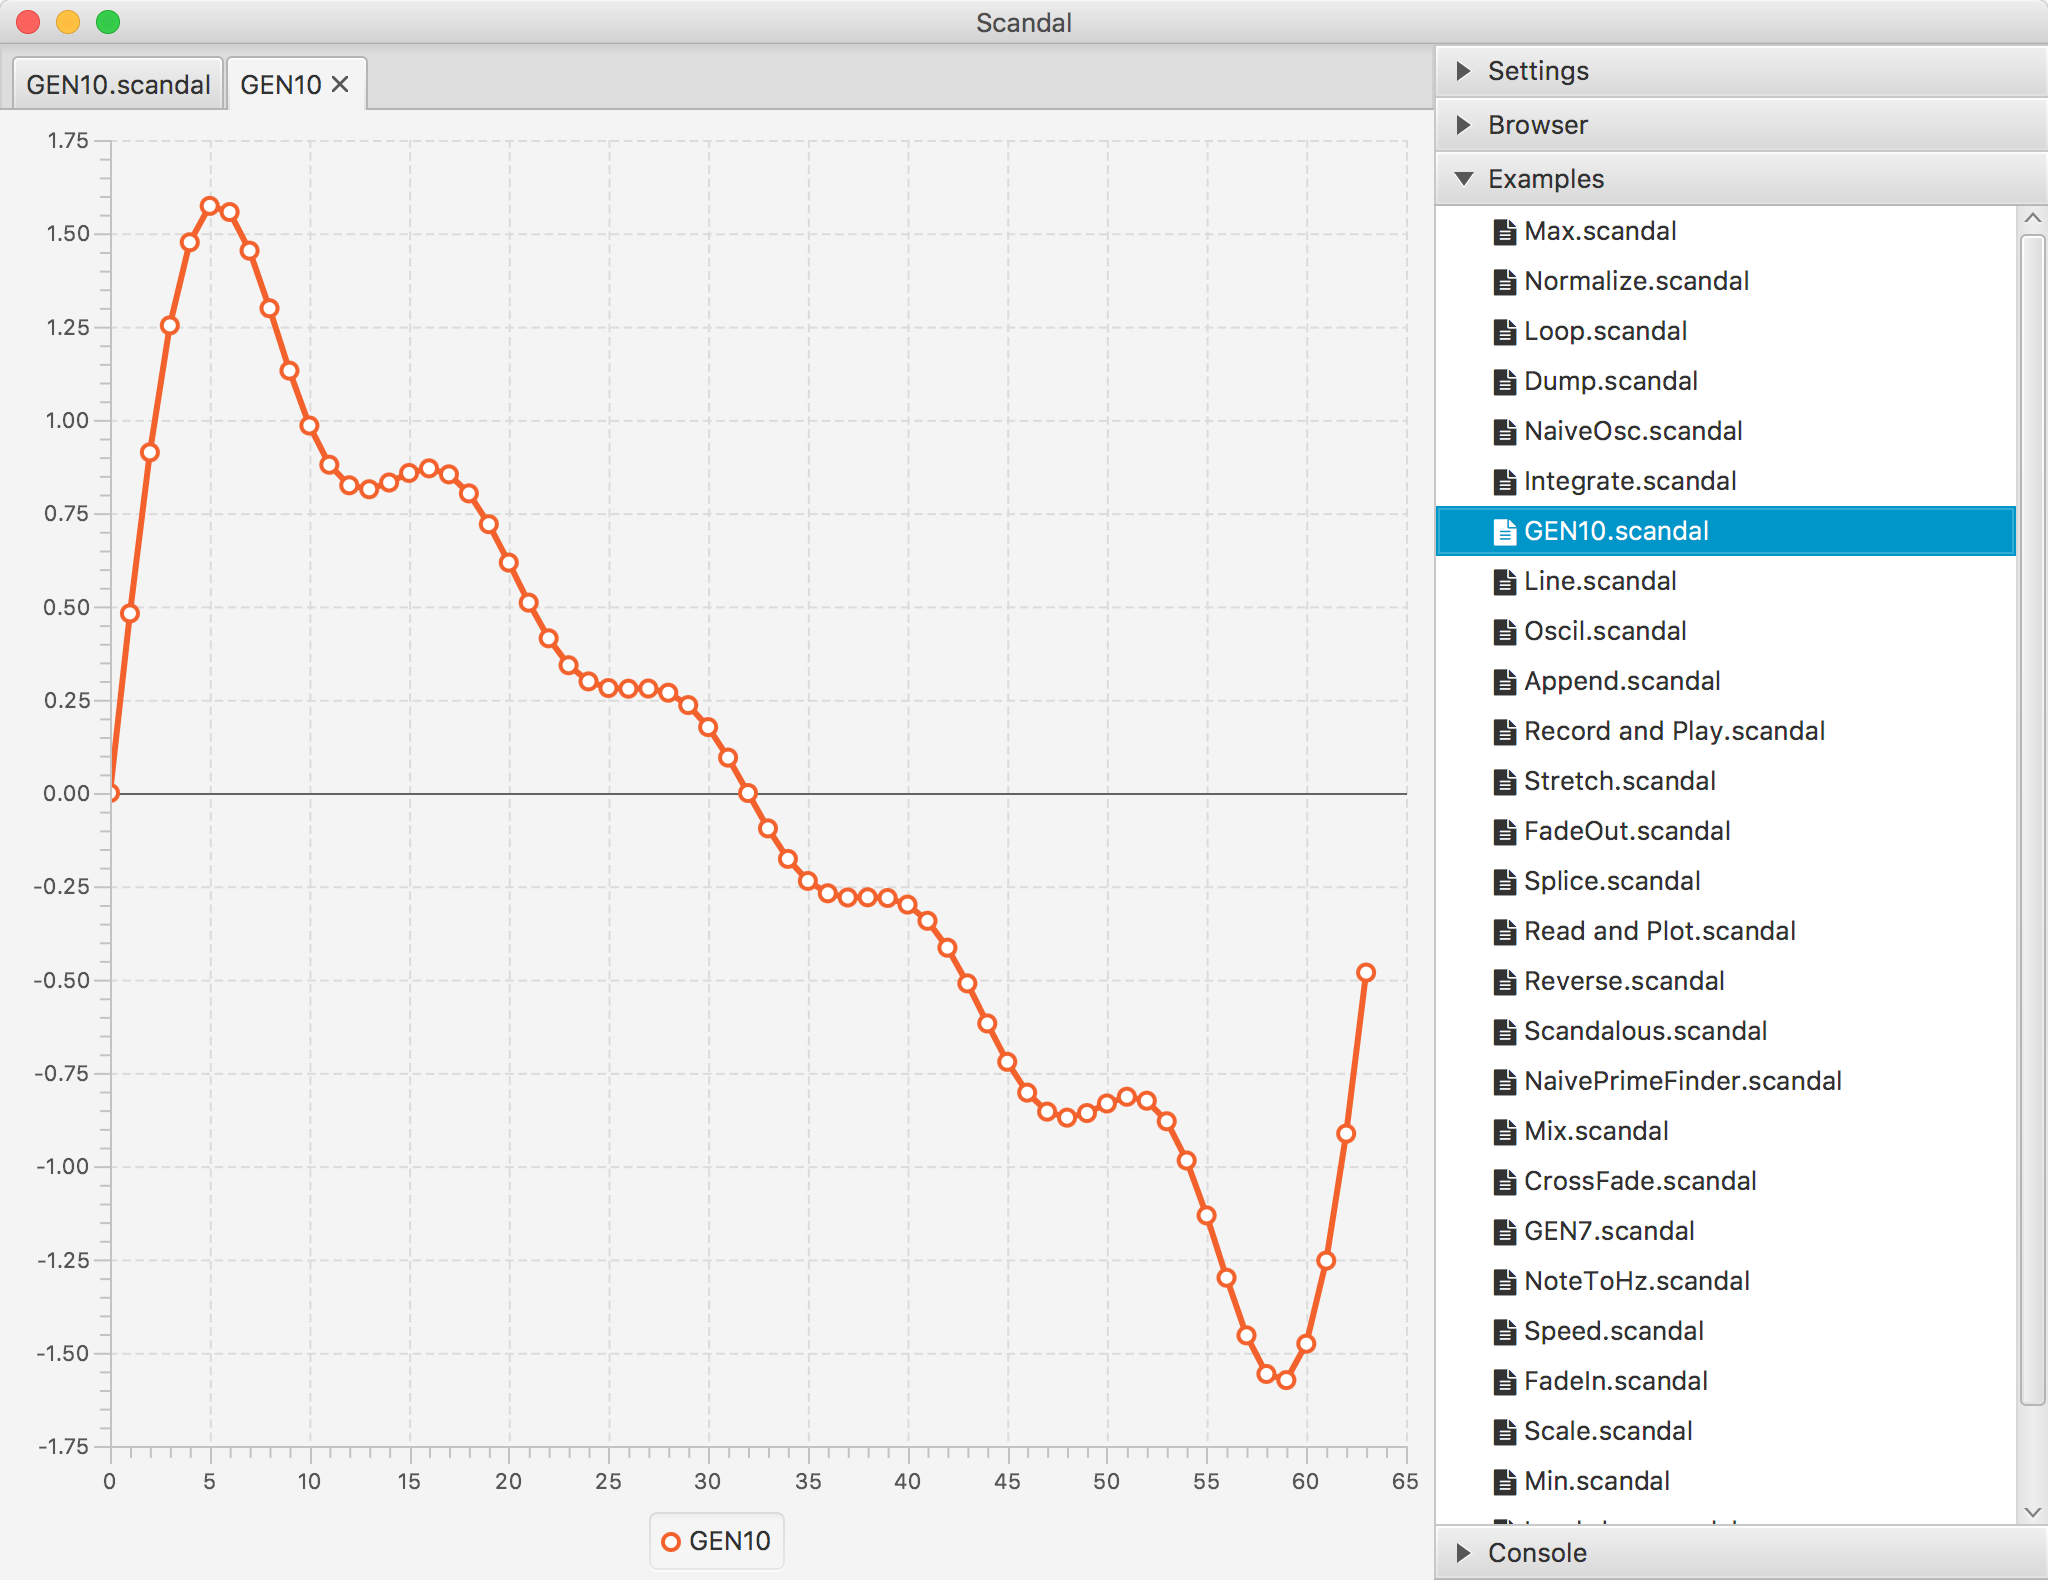
\includegraphics[width=4.5in]{img/plot}
	\caption[Plotting an array in \emph{Scandal}.]{Plotting an array in \emph{Scandal}.}
\end{figure}

\newpage

We parse plot statements by consuming the keyword and a left parenthesis, then calling \il{expression} on the parser three times, consuming the commas in between. We next consume the right parenthesis, and return an instance of \il{PlotStatement}, whose constructor uses the keyword token and first expression to construct the superclass. Decoration of a plot statement is accomplished simply by asking each expression to decorate itself. We then type-check the first to be a string, the second to be an array, and overload the third to accept integers and floats. The generation phase checks, like we did with print statements, if we are running on the IDE. If not, we do not generate any bytecode, hence one cannot plot when running a \emph{Scandal} program from the command line. Otherwise, we use \il{mv} to push a new instance of \il{language.ide.PlotTab}, and push all three expressions on top of it. If the last expression has type float, we give the \il{F2I} instruction, and finally call \il{init} on the \il{PlotTab}, causing it to be displayed in the main view. We provide a thorough discussion of \emph{Scandal}'s IDE in the next chapter.

Play statements take an array of audio samples and an integer number of channels, hence extend \il{Statement} by adding to id a second expression property. Parsing is done exactly the same way it is for plot statements, only we have here one less expression to parse. Decoration follows the same pattern, and requires that the first expression be an array, and the second be an integer. We here choose not to overload the integer expression, although it may be useful in the future to use floats in order to define a surround configuration, such as 5.1, or 8.4 speakers, where the decimal part corresponds to the number of sub-woofers in a speaker configuration. Like before, we check in the generation phase whether we are running inside the IDE. If not, we use \il{mv} to push a new instance of \il{AudioTask} onto the stack, then duplicate it, since we are using it twice. We then call \il{init} on the \il{AudioTask}, which pops the topmost of the two. We then generate both expressions, call \il{play} on the \il{AudioTask}, and return. If we are on the IDE, however, we push instead a new instance of \il{language.ide.WaveTab}. We then push a string containing the class name, which the symbol table holds, generate both expressions, and call \il{init} on the \il{WaveTab}. The string containing the class name is used as the tab's label. The \il{WaveTab} class in the IDE is a subclass of \il{PlotTab}, hence displays a plot of the array of samples, decimated to 1000 samples, in addition to playing it back, hence there one never needs to plot \il{and} play in a \emph{Scandal} program.

The last type of framework statement in the language deals with saving a \emph{.wav} file to disk. Write statements take three arguments, namely the array containing audio samples, a string containing a path in the file system, and an integer number of channels. Parsing follows the same methodology of other framework statements, so does decoration. We do not overload the channel count, but we might in the future to support surround configurations, similarly to play statements. The code-generation routine uses \il{mv} to push a new instance of \il{framework.generators.AudioTask}, which we duplicate. We will discuss the audio engine's framework package in the next chapter. After calling \il{init} on the \il{AudioTask}, we push all expressions and \il{export} on \il{AudioTask}, which effectively saves the audio buffer as a \emph{.wav} at the specified path. We summarize below the type-checker rules for all subclasses of \il{Statement}.

\begin{itemize}
	\item ImportStatement:
		\begin{itemize}
			\item Must be stated in the outermost scope
			\item Expression.type = Types.\texttt{STRING}
		\end{itemize}
	\item AssignmentStatement:
		\begin{itemize}
			\item Must have been declared in some enclosing scope
			\item Declaration.Type = Expression.type
		\end{itemize}
	\item IndexedAssignmentStatement:
		\begin{itemize}
			\item Must have been declared in some enclosing scope
			\item Declaration.Type = Types.\texttt{ARRAY}
			\item Expression\_0.type = Types.\texttt{INT} $|$ Types.\texttt{FLOAT}
			\item Expression\_1.type = Types.\texttt{INT} $|$ Types.\texttt{FLOAT}
		\end{itemize}
	\item IfStatement:
		\begin{itemize}
			\item Expression.type = Types.\texttt{BOOL}
		\end{itemize}
	\item WhileStatement:
		\begin{itemize}
			\item Expression.type = Types.\texttt{BOOL}
		\end{itemize}
	\item PrintStatement:
		\begin{itemize}
			\item Expression.type != Types.\texttt{ARRAY} $|$ Types.\texttt{LAMBDA}
		\end{itemize}
	\item PlotStatement:
		\begin{itemize}
			\item Expression\_0.type = Types.\texttt{STRING}
			\item Expression\_1.type = Types.\texttt{ARRAY}
			\item Expression\_2.type = Types.\texttt{INT} $|$ Types.\texttt{FLOAT}
		\end{itemize}
	\item PlayStatement:
		\begin{itemize}
			\item Expression\_0.type = Types.\texttt{ARRAY}
			\item Expression\_1.type = Types.\texttt{INT}
		\end{itemize}
	\item WriteStatement:
		\begin{itemize}
			\item Expression\_0.type = Types.\texttt{ARRAY}
			\item Expression\_1.type = Types.\texttt{STRING}
			\item Expression\_2.type = Types.\texttt{INT}
		\end{itemize}
\end{itemize}

\subsection{Subclasses of \il{Expression}}

Expressions in \emph{Scandal} cannot be evaluated on their own, rather existing only in the context of a declaration or statement. The abstract class \il{Expression} has a very diverse family of subclasses, and extends \il{Node} by adding three static methods. These methods are type converters and will be discussed in the context of lambda expressions. \il{Expression} neither implements \il{decorate} or \il{generate}, nor adds any properties to \il{Node}, hence remaining a fairly general type of node. Given their diversity, and the fact that often expressions come as binary sub-trees of the AST, expressions are by very far the most difficult construct in the language to parse. The \il{expression} routine in the parser works by always looking for operator tokens, then forming a binary expression whenever applicable. Hence even when a simple literal expression is given, parsing thereof goes through several steps before delegating to the specific parsing routine for that particular type of literal. The concrete syntax rules for the various types of expressions reflect this fact in the sense that \emph{every} subclass of \il{Expression} is treated while parsing as a binary tree, even if it eventually turns out to be a trivial, single-leaf tree. The leaves are called factors in the production rules below. Above factors, there can be summands, and above summands there can be comparisons, depending on the precedence of the connecting operators. In \emph{Scandal}, we do not allow carets or double-stars for exponentiation. Should we do allow them in the future, they would need to be introduced in the rules below with a higher precedence than factors, that is, powers would need to replace factors as leaves.

\begin{itemize}
	\item expression := comparison (comparisonOp comparison)$^*$
	\item comparisonOp := \texttt{LT} $|$ \texttt{LE} $|$ \texttt{GT} $|$ \texttt{GE} $|$ \texttt{EQUAL} $|$ \texttt{NOTEQUAL}
	\item comparison := summand (summandOp summand)$^*$
	\item summandOp := \texttt{PLUS} $|$ \texttt{MINUS} $|$ \texttt{OR}
	\item summand := factor (factorOp factor)$^*$
	\item factorOp := \texttt{TIMES} $|$ \texttt{DIV} $|$ \texttt{MOD} $|$ \texttt{AND}
	\item factor := derivedExpression $|$ literalExpression $|$ arrayExpression
	\item factor := frameworkExpression $|$ lambdaExpression
\end{itemize}

We begin parsing expressions by assuming the expression given is a binary expression containing a lowest-precedence comparison operator. Inside the \il{expression} routine in the parser, we create two expressions, one for each node of the binary sub-tree whose root we are attempting to create. We then ask the \il{comparison} routine to provide us with the left-hand side expression and test in a while-loop to see whether the next token is a comparison operator. If so, we ask \il{comparison} for the right-hand side expression and create an instance of \il{BinaryExpression} with the two expressions. While the next token is still a comparison operator, we keep asking \il{comparison} for a new right-hand side, then substitute our instance of \il{BinaryExpression} with another in which the left-hand side is the entire binary expression we parsed last, and the right-hand side is the last expression returned from the \il{comparison} method. In this fashion, we always associate equal-precedence operations from left to right. The \il{expression} routine is given below in Listing \ref{alg:expr}.

\begin{lstlisting}[language=Java,caption={Parsing Expressions.},label={alg:expr}]
public Expression expression() throws Exception {
	Token firstToken = token;
	Expression e0;
	Token operator;
	Expression e1;
	e0 = comparison();
	while (token.isComparison()) {
		operator = consume();
		e1 = comparison();
		e0 = new BinaryExpression(firstToken, e0, operator, e1);
	}
	return e0;
}
\end{lstlisting}

Inside \il{comparison}, we do exactly the same we do inside \il{expression}, only we check whether the operator token is at the precedence level of sums. We instantiate expressions inside \il{comparison} by calling the \il{summand} routine. The \il{summand} routine, in turn, does also exactly the same as \il{expression} and \il{comparison}, only checking whether operator tokens are at precedence level of products, which is the highest level of precedence among operator tokens in \emph{Scandal}. Inside \il{summand}, we instantiate expressions by calling the \il{factor} routine. The latter returns a leaf in the binary tree by looking at the FIRST set of the \il{expression} rule, similarly to how we parse declarations and statements. Some factors, however, require more than one token of look-ahead, namely some of those that begin with an identifier. Inside the \il{factor} routine, then, whenever we see a token of kind \texttt{IDENT}, we look for the next token to determine whether we should parse the factor as an indexed array, a lambda application, a lambda composition, or simply an identifier expression. It turns out two tokens of look-ahead is enough to parse factors, which thus have a LL(2) grammar. We have the following abstract syntax rules for expressions, wherein the rules for operators are the same as the concrete rules, except that instead of strings of characters, we have instances of \il{Token}.

\begin{itemize}
	\item Expression := DerivedExpression $|$ LiteralExpression $|$ ArrayExpression
	\item Expression := FrameworkExpression $|$ LambdaExpression $|$ BinaryExpression
	\item BinaryExpression := Expression\_0 Operator Expression\_1
	\item Operator := ComparisonOperator $|$ SummandOperator $|$ FactorOperator
\end{itemize}

\subsubsection{The \il{BinaryExpression} Class}

Binary expressions extend \il{Expression} by overriding its abstract methods and adding three properties, namely a left-hand side expression, an operation token, and a right-hand expression. Decorating and generating binary expressions is somewhat involved, mostly due to the great variety of operations and their supported types. In addition, operators in \emph{Scandal} are overloaded to a certain extent, as to provide type polymorphism in binary expressions, which adds to the number of cases with which we must deal in decorating and generating expressions, but also make the DSL more concise and readable. Decorating a binary expression begins with asking both expressions to decorate themselves, after which their types will be non-null. Given the binary-tree nature of these expressions, this is accomplished recursively, hence we may be calling \il{decorate} on ourselves if one of the sub-expressions is itself a binary expression. Hence we need to have a type before returning from \il{decorate}. As a matter of fact, almost all we do next inside \il{decorate} is go over the different combinations of operations and types to determine what the overall type of the binary expression is. If we are given two expressions in any combination of integers or floats, we can perform arithmetic on those numbers. Note that arithmetic operators do not always have the same precedence amongst themselves. We then have two sub-cases. If both expressions are of type integer, then we decorate the resulting binary expression with an integer type. Otherwise, if at least one of the expressions has type float, the whole binary expression will have type float. If instead we are given any combination of integers, floats, or booleans, then we can use logical or comparison operators, remembering that booleans are implemented in bytecode as integers, and that logical operators also have different precedence levels. In both cases, the binary expression will be of type boolean. Before returning, we need to deal with the caveat of having applications of lambdas that were declared as parameters of another lambda. Given that there is no parameterization of types in \emph{Scandal}, these lambdas must be applied alone first in an assignment declaration, which is the current inference mechanism for such parameterized types. So we check both expressions to see whether their declaration is a subclass of \il{ParamDeclaration}, and throw an error if that is the case. The very last thing we do while decorating a binary expression is check if our type is still null. If so, all test above have failed. Since we must decorate the expression with a type, an error is thrown whenever type-checking fails.

Generating binary expressions is even more involved, given that operators are \emph{not} overloaded in bytecode at all, hence we need to do all the work. The basic mechanism is to load the left expression, then create a case for each kind of operator. The procedure for all arithmetic operators is very similar. After pushing the left expression, we check if the binary expression has type float. If so, we know at least one of the expressions must have type float. So while the left expression is still on top of the stack, we check if it is \emph{not} a float, and if so call the \il{I2F} instruction. We then push the right expression and do the same check. The last step is to call the appropriate JVM instruction to deal with the float case of the arithmetic operator at hand. If, on the other hand, the binary expression has integer type, then we know \emph{both} expressions also have integer type, so we just push the second expression and call the appropriate JVM instruction. In the cases where we have a logical operator, we observe that the JVM can only perform logical operations on integers, including naturally integer representations of booleans. So here we load the left expression and cast it to integer if it is a float, do the same for the right expression, and call the logical operator's instruction. Comparison operators are more tricky, since we cannot count on the overall type of the binary expression to make necessary conversions, and the JVM does have separate instructions for integers and floats, provided both sides have the same type. Every binary expression whose operator is a comparison has type boolean, but still, JVM instructions are not overloaded, hence we need to have agreeing types on top of the stack before calling a particular instruction. However, observing that after calling the operator instruction, we are always left with an expression of type boolean on top of the stack, we work around testing every possible case by casting both expressions to float, as needed, and only resorting to float comparisons.

Overloading operators can be very beneficial for a DSL. \emph{MATLAB} is perhaps one of the best examples, but also \emph{Csound} operates almost exclusively on overloaded array operations. Expressions that resemble the way we write them mathematically are also fundamental in improving readability, as well as removing the clutter created by words that have a household symbolic representation. The future steps of \emph{Scandal} shall improve even further the functionality of binary expressions. Given the nature of the language's domain, overloaded array operations are the next logical step. As a simple example, one could apply a scalar to an entire array in the same way we write such an expression mathematically. Let $\alpha = 2$ and $\vec{v} = [1 \; 2 \; 3]$. Then $\alpha \cdot \vec{v} = [2 \; 4 \; 6]$. With overloaded array operations, one could write \il{a * [1, 2, 3]} and have it evaluated to \il{[2, 4, 6]}.

\subsubsection{Derived Expressions}

\begin{itemize}
	\item derivedExpression := parethesizedExpression $|$ unaryExpression $|$ identExpression
	\item parethesizedExpression := \texttt{LPAREN} expression \texttt{RPAREN}
	\item unaryExpression := (\texttt{KW\_MINUS} $|$ \texttt{KW\_NOT}) expression
	\item identExpression := \texttt{IDENT}
\end{itemize}












% \subsubsection{Literal Expressions}

% Literal expressions are the simplest constructs in the language, and have the following concrete rules:

% \begin{itemize}
% 	\item literalExpression := intLitExpression $|$ floatLitExpression
% 	\item literalExpression := boolLitExpression $|$ stringLitExpression
% 	\item intLitExpression := \texttt{INT\_LIT}
% 	\item floatLitExpression := \texttt{FLOAT\_LIT}
% 	\item boolLitExpression := \texttt{KW\_TRUE} $|$ \texttt{KW\_FALSE}
% 	\item stringLitExpression := \texttt{STRING\_LIT}
% \end{itemize}

% In the productions above, we note that non-zero integer literals are not allowed to start with a zero. In such a scenario, even though the scanner will create two tokes, one for zero, and another for the rest of the number, since there are no productions in the language that take two integers separated by white space, the parser inevitably will throw a compilation error. The same applies to floating-point decimals, where only one zero can come before the dot. I this particular case, a zero actually \emph{must} precede the \texttt{DOT} token, and such constructs as $x = .5$ are not allowed. Doubles, shorts, or longs do not exist in \emph{Scandal} as of yet, and there is no need to declare float literals the way they are in \emph{Java}, with $1.1f$ for float and $1.1$ for double, say. In fact, that will throw an error. As previously mentioned, string literals are constructed by enclosing text within quotes, and the use of apostrophes will cause a scanning error. Even though quotes are in the language's alphabet, they are never converted into a \il{Token}, as their only possible use is within a string literal. \texttt{DOT}, on the other hand, has uses besides separating the decimal part of a \texttt{FLOAT\_LIT}, namely in composed lambdas. Hence the scanner simply instantiates a token and delegates the inferring of meaning to the parser. Boolean literals are quite self-explanatory, and unlike \emph{C}, numbers are not allowed to replace booleans.

% \subsubsection{Array Expressions}

% \begin{itemize}
% 	\item arrayExpression := arrayLitExpression $|$ arrayItemExpression
% 	\item arrayExpression := arraySizeExpression $|$ newArrayExpression
% 	\item arrayLitExpression := \texttt{LBRACKET} expression (\texttt{COMMA} expression)$^*$ \texttt{RBRACKET}
% 	\item arrayItemExpression := identExpression \texttt{LBRACKET} expression \texttt{RBRACKET}
% 	\item arraySizeExpression := \texttt{KW\_SIZE} \texttt{LPAREN} expression \texttt{RPAREN}
% 	\item newArrayExpression := \texttt{KW\_NEW} \texttt{LPAREN} expression \texttt{RPAREN}
% \end{itemize}

% \subsubsection{Framework Expressions}

% \begin{itemize}
% 	\item frameworkExpression := piExpression $|$ cosExpression $|$ powExpression
% 	\item frameworkExpression := floorExpression $|$ readExpression $|$ recordExpression
% 	\item piExpression := \texttt{KW\_PI}
% 	\item cosExpression := \texttt{KW\_COS} \texttt{LPAREN} expression \texttt{RPAREN}
% 	\item powExpression := \texttt{KW\_POW} \texttt{LPAREN} expression \texttt{RPAREN}
% 	\item floorExpression := \texttt{KW\_FLOOR} \texttt{LPAREN} expression \texttt{RPAREN}
% 	\item readExpression := \texttt{KW\_READ} \texttt{LPAREN} expression \texttt{COMMA} expression \texttt{RPAREN}
% 	\item recordExpression := \texttt{KW\_RECORD} \texttt{LPAREN} expression \texttt{RPAREN}
% \end{itemize}

% \subsubsection{Lambda Expressions}

% \begin{itemize}
% 	\item lambdaExpression := lambdaApp $|$ lambdaComp $|$ lambdaLit $|$ lambdaBlock
% 	\item lambdaApp := identExpression \texttt{LPAREN} expression (\texttt{COMMA} expression)$^*$ \texttt{RPAREN}
% 	\item lambdaComp := identExpression (\texttt{DOT} identExpression)$^*$
% 	\item lambdaComp := identExpression (\texttt{DOT} identExpression)$^*$ \texttt{DOT} lambdaApp
% 	\item lambdaLit := paramDeclaration \texttt{ARROW} (paramDeclaration \texttt{ARROW})$^*$ expression
% 	\item lambdaBlock := paramDeclaration \texttt{ARROW} (paramDeclaration \texttt{ARROW})$^*$ retBlock
% 	\item retBlock := \texttt{LBRACE} (assignmentDeclaration $|$ statement)$^*$ retExpression \texttt{RBRACE}
% 	\item retExpression := \texttt{KW\_RETURN} expression
% \end{itemize}